\documentclass{exam}

\usepackage{amsmath,amssymb,amsfonts,amsthm,dsfont}
\usepackage{lib/extra}
\usepackage{graphicx}
\usepackage{tikz}
\usepackage{enumitem}
\usepackage{bbm}
\usepackage{pgfplots}
\usepackage{fontenc}
\usepackage{float}

\pgfplotsset{compat=1.18}

\title{ECE 569 HW 2}
\author{Brandyn Tucknott}
\date{Due 28 October 2025}

\newcommand{\new}{\text{new}}
\newcommand{\sign}{\text{sign}}
\newcommand{\conv}{\text{conv}}
\newcommand{\redconv}{\text{ReducedConv}}
\newcommand{\ans}{\text{\textbf{\underline{Answer:} }}}

\begin{document}
\maketitle

\begin{questions}
    % Question 1
    \question (Geometry of SVM) Consider the training samples $\cbrac{x_i, y_i}$. Suppose that the training samples are from two
    classes. Let us denote the samples as $\mathcal{A}\subseteq \R^n$ (class label +1) and $\mathcal{B}\subseteq\R^n$ (class label -1)
    where $\mathcal{A}\cup\mathcal{B} = \cbrac{x_1, \hdots, x_n}$. SVM aims to find a hyperplane that can separate the convex hulls
    of $\mathcal{A} = \cbrac{a_1, \hdots, a_m}$ and $\mathcal{B} = \cbrac{b_1, \hdots, b_k}$ in the $n$-dimensional space.
    \begin{parts}
        % part a
        \part $\brac{\textbf{Existence}}$ When does such a hyperplane exist; i.e., under what geometry of the training set does the
        SVM classifier exist? (use convex theory to support your answer)

        \ans Such a hyperplane exists when $\conv \mathcal{A}$ and $\conv \mathcal{B}$ are disjoint. 


        % part b
        \part $\brac{\textbf{Generalization}}$ After a hyperplane is learned, say $w^Tx = c$, which satisifies
        $$w^Ta_i \leq c \text{ for all }a_i\in\mathcal{A} \quad w^Tb_k > c \text{ for all }b_k\in \mathcal{B}.$$
        The prediction is as follows:
        $$\hat{y}_\new = \sign (c - w^Tx_\new),$$
        where $x_\new$ is unseen test data and $\hat{y}_\new$ is the predicted label. Consider the two hyperplanes in the figure.
        Which one do you prefer to have better performance in the prediction stage? Explain.

        \begin{figure}[H]
            \centering
            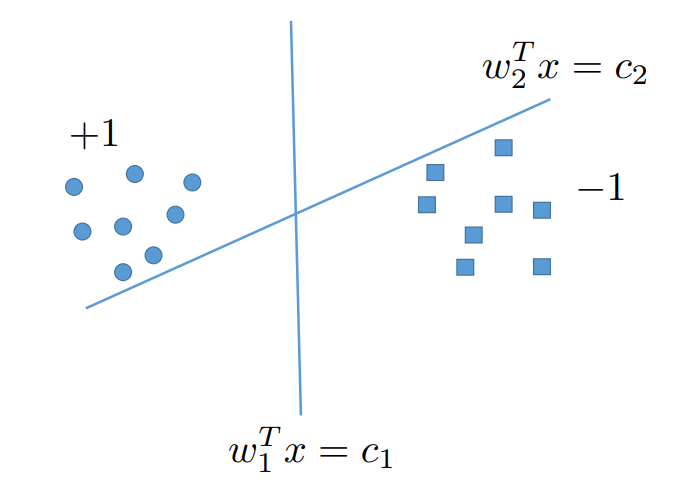
\includegraphics[scale=.5]{figures/school_work/ECE_569/HW_2/figure1.png}
        \end{figure}
        \ans Call the hyperplanes $H_1 := w_1^Tx = c_1$ and $H_2 := w_2^Tx = c_2$. For this particular example, 
        we prefer to use the classifier given by $H_1$ since if we use $H_2$ it is possible to have a point near the $+1$ cluster and far from the $-1$ cluster
        still get classified as $-1$. In a sligtly more mathematical sense, $H_1$ has a larger margin, so it has a larger room for error and is therefore the better choice.
    \end{parts}


    \newpage
    % Question 2
    \question (Problem Formulation of SVM) The rationale behind finding a good separating hyperplane for $\mathcal{A}$ and $\mathcal{B}$ is as follows:
    \begin{enumerate}
        \item Find convex hulls of $\mathcal{A}$ and $\mathcal{B}$.

        \item Find points $c^*$ and $d^*$ from conv $\mathcal{A}$ and conv $\mathcal{B}$ respectively, and they are the closest to each other.

        \item Construct a line segment between the two points.

        \item Find a hyperplane orthogonal to the line segment and passing through its midpoint.
    \end{enumerate}
    \begin{parts}
        % part a
        \part Express this as a convex optimization problem. \\
        \ans
        \begin{align*}
            \text{minimize } & \norm{Au - Bv}_2 \\
            \text{subject to } & \mathbf{1}^Tu = 1 \\
            & \mathbf{1}^Tv = 1 \\
            & u \geq 0 \\
            & v \geq 0
        \end{align*}

        All constraints of the above optimization problem are affine, and since all norms in $\R^n$ are convex,
        we conclude that it is a convex optimization problem.

        % part b
        \part Express the classifier hyperplane following steps 1-4.
        \begin{proof}
            We assume $c^*$ and $d^*$ are from $\conv\mathcal{A}$ and $\conv\mathcal{B}$ respectively and admit the smallest distance between
            the two convex hulls. To derive a hyperplane which is an orthogonal bisector to the line segment from $c^*$ to $d^*$, we wish for the following to be true:
            $$\text{for any } x \text{ on our hyperplane, } \norm{x - c^*}_2 = \norm{x - d^*}_2.$$

            We can maniuplate this equation to end up with a hyperplane.
            \begin{align*}
                \norm{x - c^*}_2 &= \norm{x - d^*}_2 \\
                \norm{x - c^*}_2^2 &= \norm{x - d^*}_2^2 \\
                x^Tx - 2x^Tc^* + c^*^Tc^* &= x^Tx - 2x^Td^* + d^*^Td^* \\
                2x^T(d^* - c^*) &= \norm{d^*}_2^2 - \norm{c^*}_2^2 \\
                (d^* - c^*)^Tx &= \frac{\norm{d^*}_2^2 - \norm{c^*}_2^2}{2}.
            \end{align*}
            This is exactly the equation of a hyperplane, so we are done.
        \end{proof}

    \end{parts}


    \newpage
    % Question 3
    \question (Alternative Problem Formulation for SVM) Instead of first finding two points and constructing the separating hyperplane,
    we can formulate the problem directly.
    \begin{parts}
        % part a
        \part What is the distance between the following two hyperplanes:
        $$w^Tx = \alpha \quad w^Tx = \beta.$$
        \ans Notice these hyperplanes are parallel because they have the same normal vector, and in HW 1 we proved that the distance between them is
        $$d = \frac{|\alpha - \beta|}{\norm{w}_2}.$$

        % part b
        \part 2-D plot of intuition.
        \begin{figure}[H]
            \centering
            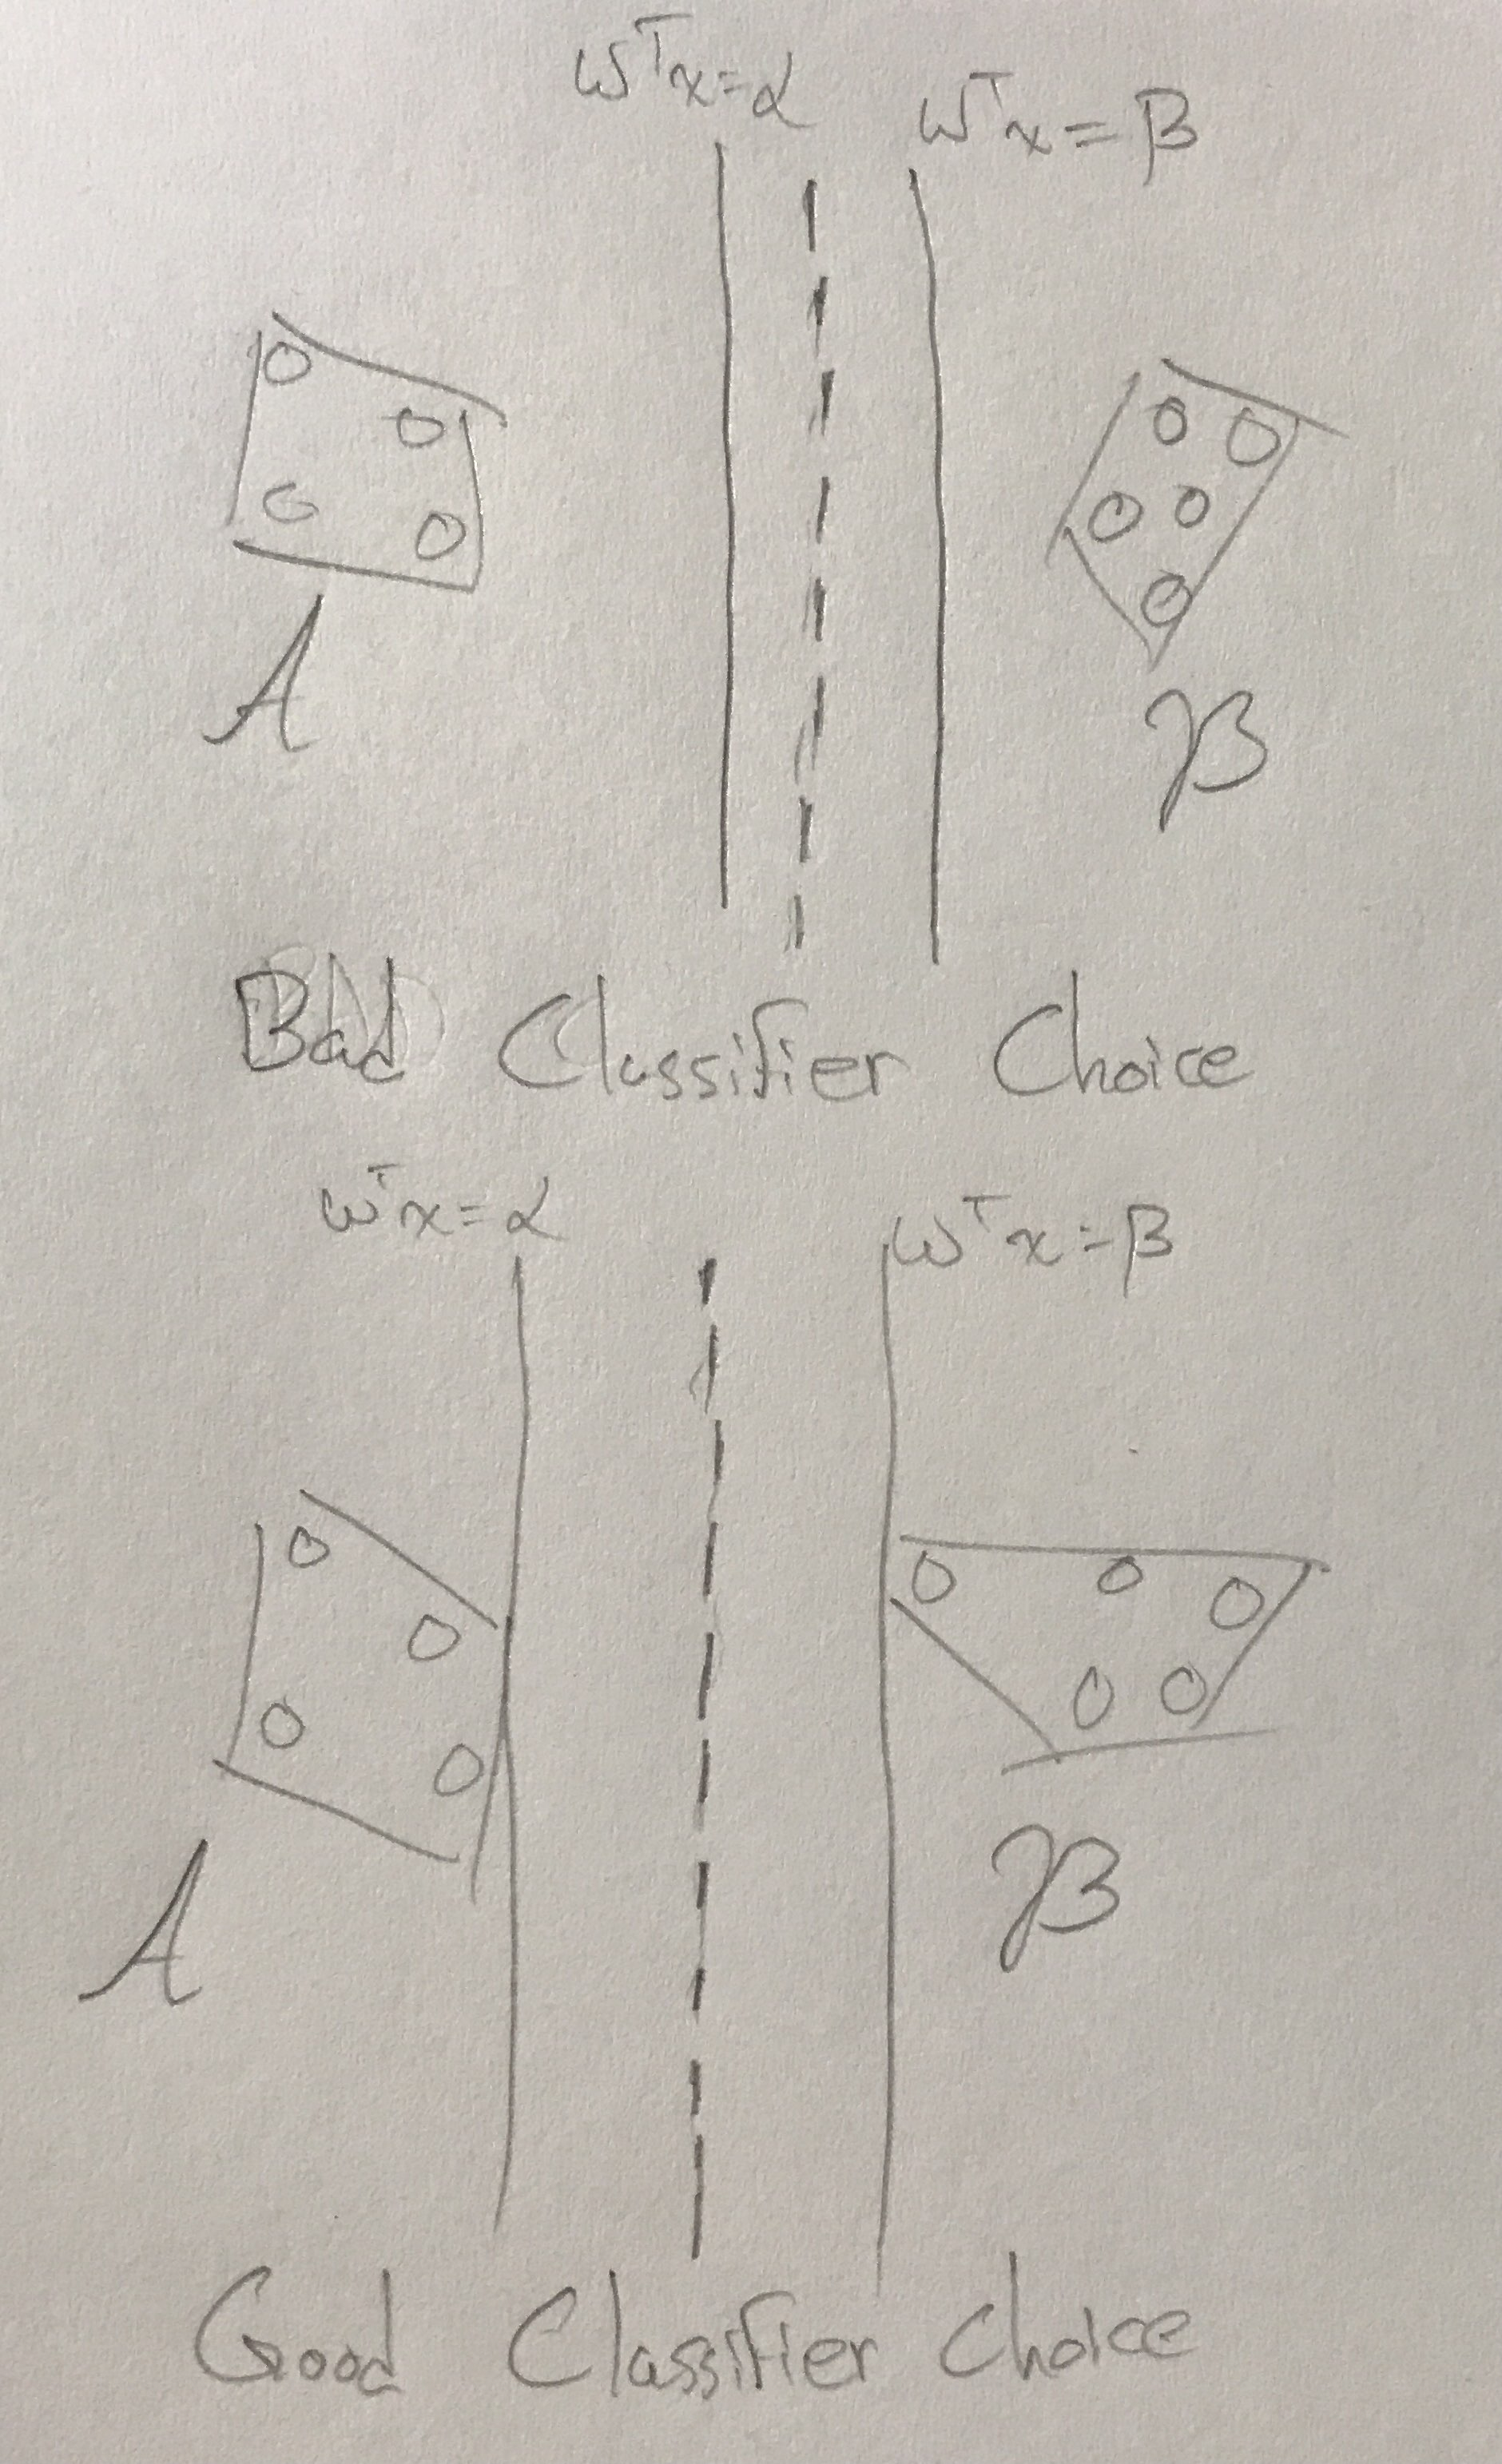
\includegraphics[scale=0.1]{figures/school_work/ECE_569/HW_2/pic1.jpg}
        \end{figure}

        % part c
        \part Formulate $w^Tx = \alpha$ and $w^Tx = \beta$ as a convex optimization problem. \\
        \ans If we assume that $\alpha \neq \beta$, then we know that $\alpha < \beta$. We wish to maximize the margin between the supporting hyper planes,
        which we know to be $|\alpha - \beta | / \norm{w}_2$. If we fix the magnitude of $w$ to be 1, we fix the scaling and can Instead
        focus on maximizing the distance itself, which is now $\beta - \alpha$. This gives us the following convex problem:
        \begin{align*}
            \text{maximize } & \beta - \alpha \\
            \text{subject to } & \norm{w}_2 = 1 \\
            & w^Ta_i \leq \alpha \\
            & w^Tb_j \geq \beta
        \end{align*}
    \end{parts}


    \newpage
    % Question 4
    \question (Robustification of SVM) Consider when conv $\mathcal{A}$ and conv $\mathcal{B}$ overlap. Define a \textbf{Reduced Convex Hull} as follows:
    $$\redconv \mathcal{A} = \cbrac{z\in \R^n : z = Au, \mathbf{1}^Tu = 1, u \geq 0, u_i \leq d, \forall i = 1, \hdots m, d\in (0, 1)}.$$
    \begin{parts}
        % part a
        \part Given the following two training sets, draw the reduced convex hull sets with $d\approx 0.8$. Explain why using reduced convex hulls
        help in the overlapping case.
        \begin{figure}[H]
            \centering
            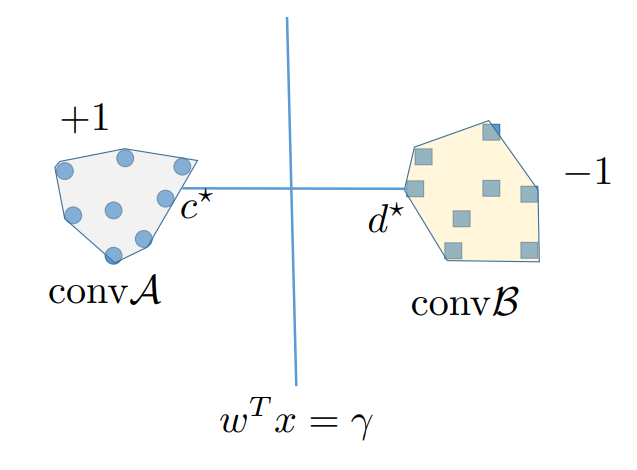
\includegraphics[scale=0.3]{figures/school_work/ECE_569/HW_2/figure2}
        \end{figure}

        \ans
        \begin{figure}[H]
            \centering
            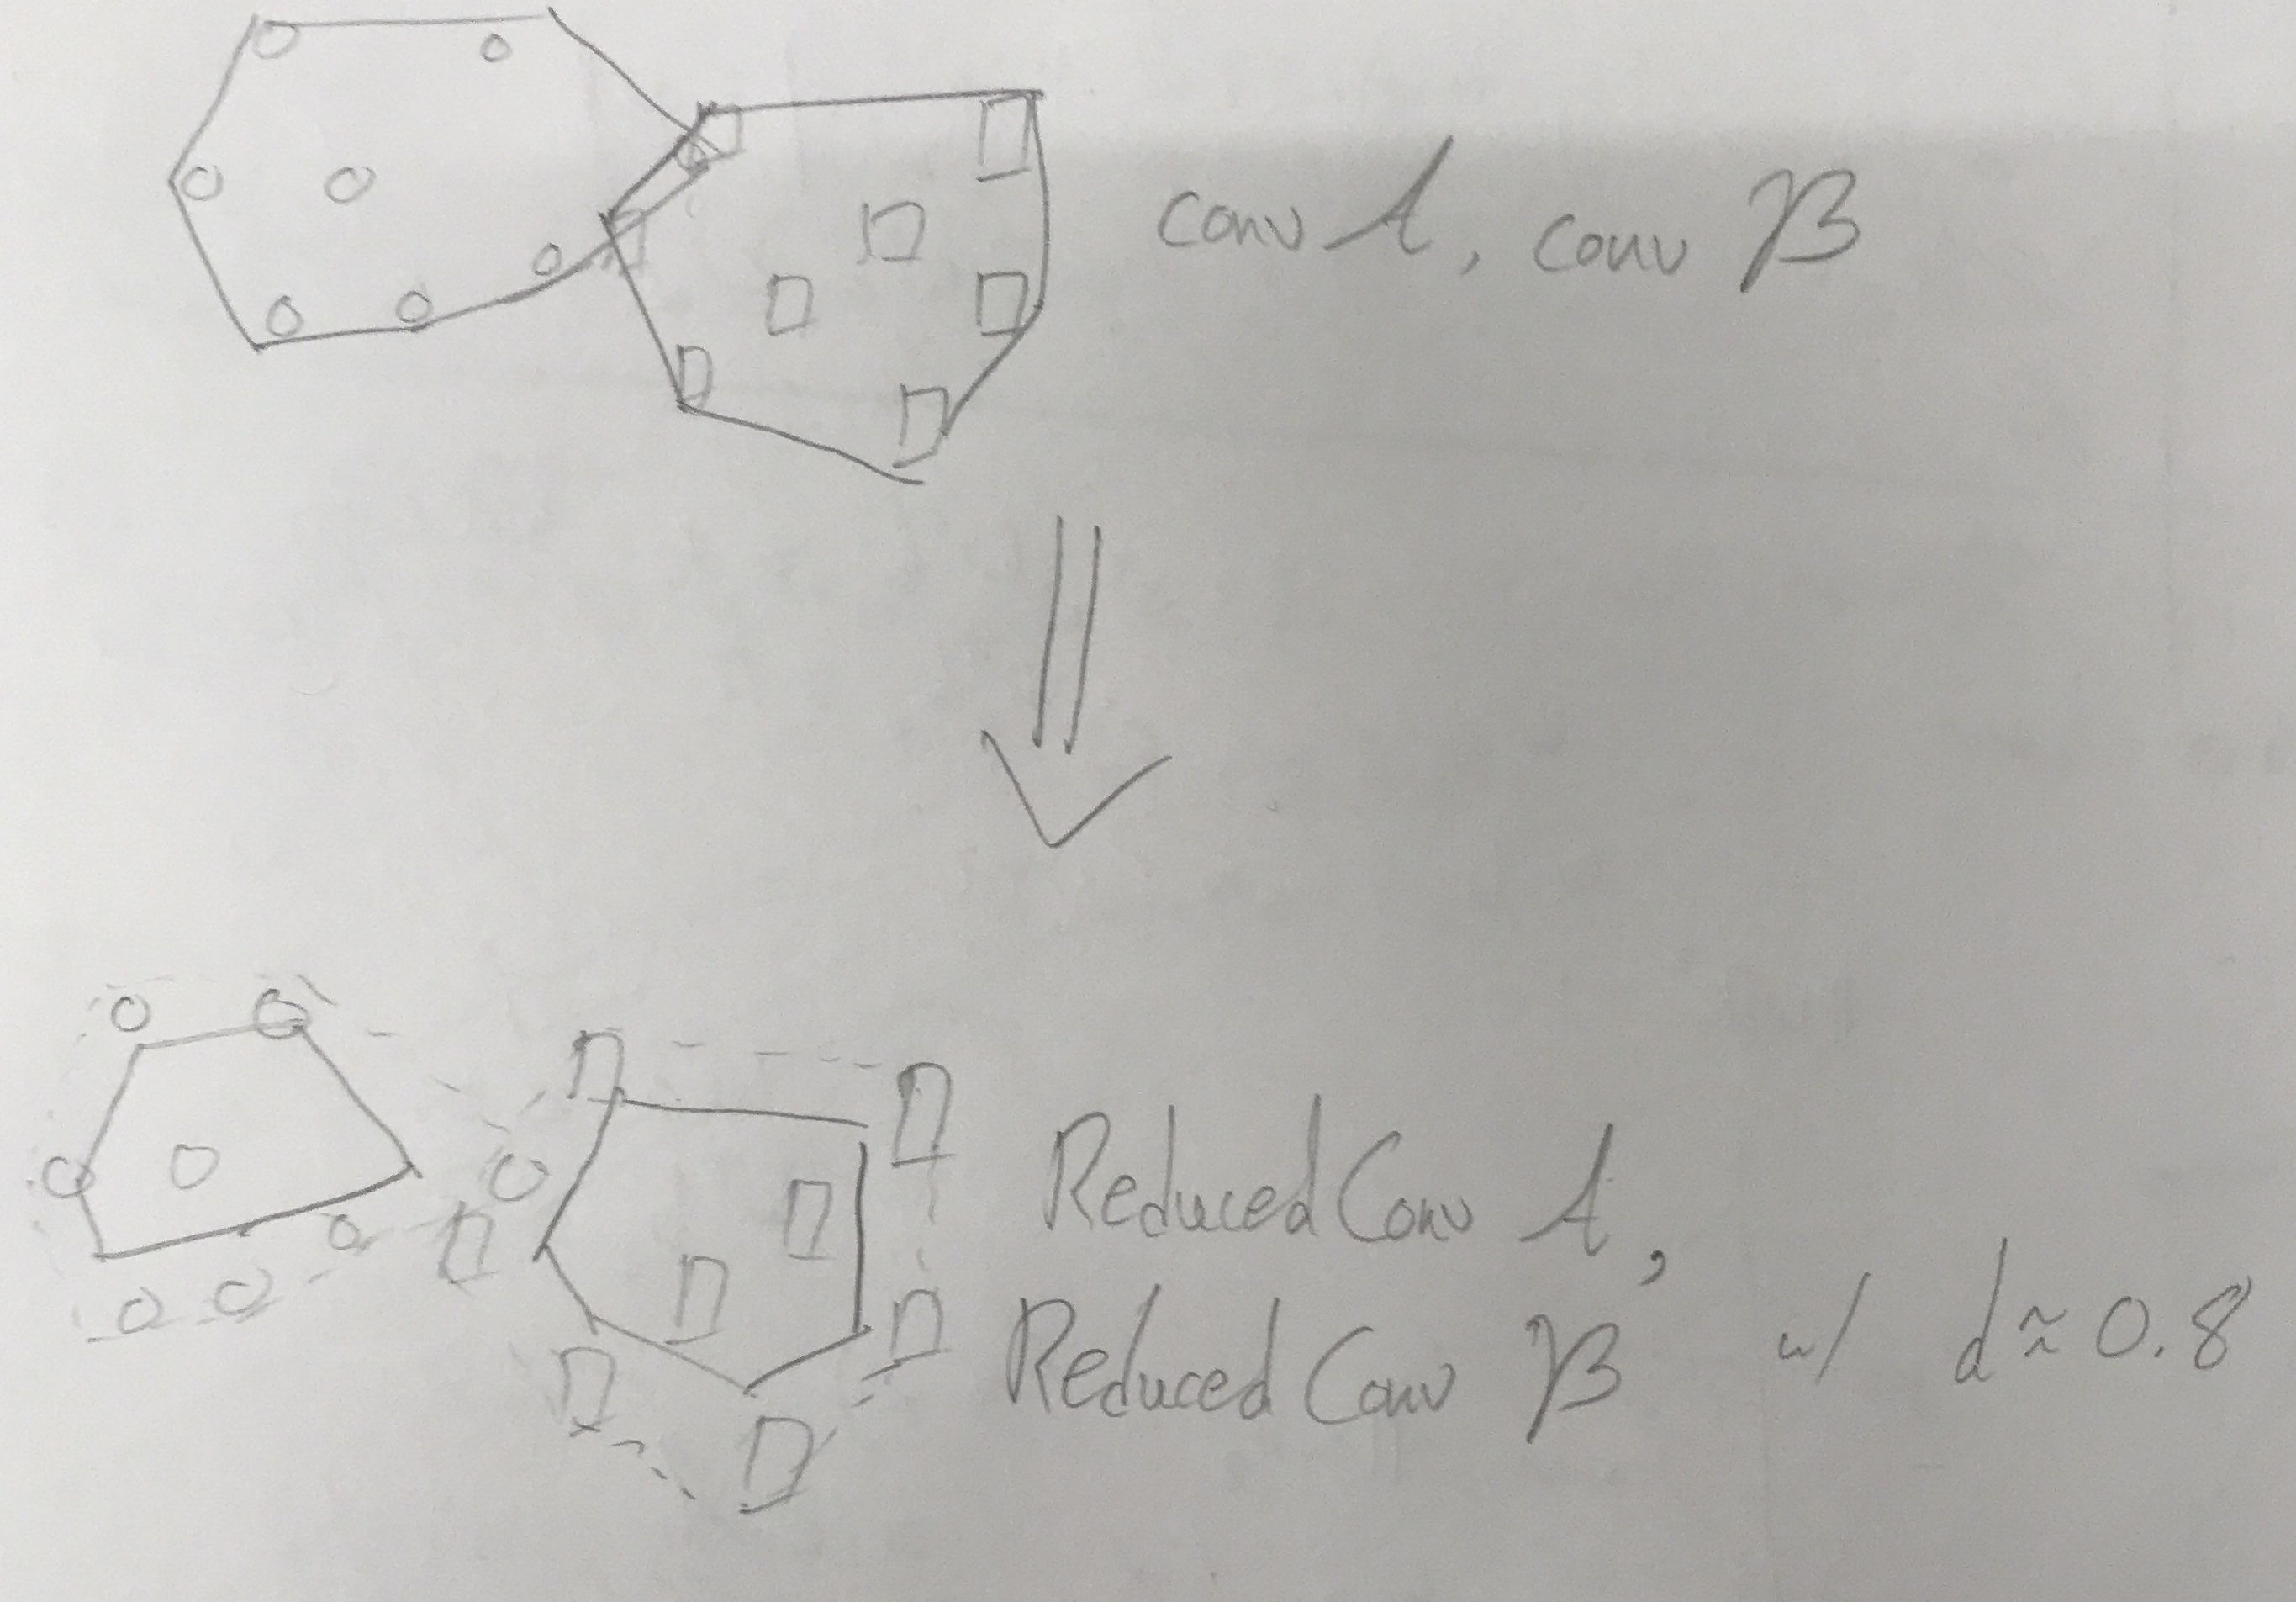
\includegraphics[scale=0.1]{figures/school_work/ECE_569/HW_2/pic2}
        \end{figure}
        The reduced convex hull is useful because with it we can define two convex subsets $\redconv\mathcal{A} \subset \conv\mathcal{A}$ and $\redconv\mathcal{B} \subset \conv\mathcal{B}$ such that
        $\redconv{A}, \redconv{B}$ are disjoint (just as in \textbf{Q2}), allowing us to use our previous formulations. Of course this won't yield a classifier which works for all datapoints, but
        it should be ``good enough". 

        % part b
        \part If the goal of the first step of the robustified SVM is to find two points from the reduced convex hulls of $\mathcal{A}$ and $\mathcal{B}$ (under prespecified $d$)
        such that the two points have the smallest distance, how do we formulate the problem? Write out your answer. Is your formulation convex? \\
        
        \ans Our answer is nearly identical to \textbf{Q2.a}, but we add the constraint $u_i, v_i \leq d$ to account for the reduced convex hull.
        \begin{align*}
            \text{minimize } & \norm{Au - Bv}_2 \\
            \text{subject to } & \mathbf{1}^Tu = 1 \\
            & \mathbf{1}^Tv = 1 \\
            & 0 \leq u \leq d \\
            & 0 \leq v \leq d
        \end{align*}

    \end{parts}


\end{questions}

\end{document}